\documentclass[12pt]{article}
\usepackage{algos-tasks}

\begin{document}
\task[regular]{Rad Enterprises}

\begin{question}
You have just been employed by Rad Enterprises to explore a system of $m$ two-way tunnels, which meet at $n$ junctions, represented as an undirected graph. Each tunnel has a particular integer level of radiation, which is between 1 and $R_\max$. Your job is to get from the entry point $e$ to a particular junction $j$, where there is a large deposit of precious metals.

Rad Enterprises is legally required to issue you with a protective suit. These suits come in different protection levels. A suit with a protection level of $p$ allows you to safely pass through tunnels with a radiation level of $p$ or less, but you will not be able to pass through tunnels with a radiation level of more than $p$.

For example, in the tunnel network below (with radiation levels shown on each tunnel), you can get from $e$ to $j$ with a suit with protection level 5; for example with the path highlighted in blue.

\begin{center}
    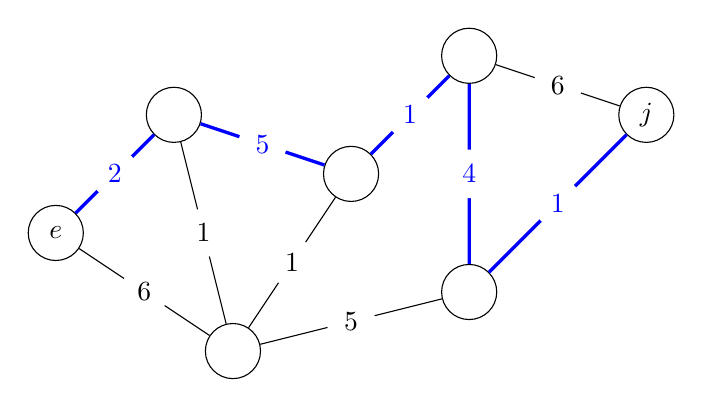
\begin{tikzpicture}[scale=1.5]
        \begin{scope}[every node/.style = {draw, circle, minimum size = 0.7cm}]
            \node (a) at (0, 0) {$e$};
            \node (b) at (1, 1) {};
            \node (c) at (1.5, -1) {};
            \node (d) at (2.5, 0.5) {};
            \node (e) at (3.5, -0.5) {};
            \node (f) at (3.5, 1.5) {};
            \node (g) at (5, 1) {$j$};
        \end{scope}
        \begin{scope}[every node/.style = {circle, fill=white}]    
        \draw (a) edge[blue, very thick] node {2} (b);
        \draw (a) edge node {6} (c);
        \draw (b) edge node {1} (c);
        \draw (b) edge[blue, very thick] node {5} (d);
        \draw (c) edge node {1} (d);
        \draw (c) edge node {5} (e);
        \draw (d) edge[blue, very thick] node {1} (f);
        \draw (e) edge[blue, very thick] node {4} (f);
        \draw (e) edge[blue, very thick] node {1} (g);
        \draw (f) edge node {6} (g);
        \end{scope}
    \end{tikzpicture}
\end{center}

Since suits with a higher protection level are more expensive, Rad Enterprises would like to work out the lowest protection level they can get away with. In the example above, the lowest protection level possible is 4, so any suit with a smaller protection level would not allow you to reach $j.$

\begin{enumerate}
    \item Design an algorithm which runs in $O(n + m)$, and decides whether you can get from $e$ to $m$ if you have a suit with a protection level of $p$.

    \textbf{Hint:} If we have a suit with protection level $p$, what edges can we definitely not traverse? 
    
    \item Hence, design an $O((n+m) \log R_{\max})$ algorithm which determines the lowest level of protection you need to get from $e$ to $j$.

    \textbf{Hint: } If you can get from $e$ to $j$ with a protection level of $p$, can you get from $e$ to $j$ with a protection level of $p+1$? Why, or why not? 
    
    \textbf{Hint: } If we \textbf{can't} reach $j$ with a protection level of $p$, what does this say about our ability to reach $j$ with a protection level of $p-1$?
\end{enumerate}
\end{question}

\begin{rubric}
\begin{enumerate}
    \item \begin{itemize}
        \item Give an $O(n+m)$ algorithm that answers `yes' if you can reach $j$ from $e$ with a protection level of $p$, and answers `no' otherwise.
        \item Briefly justify that your algorithm is correct, and runs in $O(n + m)$.
        \item Expected length: one short paragraph.
    \end{itemize} 
    \item \begin{itemize}
        \item Design an $O((n+m) \log R_{\max})$ algorithm that finds the smallest $p$ such that you can get from $e$ to $j$ with a protection level of $p$.
        \item Justify the correctness of your algorithm.
        \item Justify that your algorithm runs in $O((n+m) \log R_{\max})$ time.
    \end{itemize}
\end{enumerate}
Expected length: not more than a page.
\end{rubric}

\begin{solution}
\end{solution}

\begin{attribution}
\end{attribution}

\end{document}